\section*{Βήμα 10}

Στο βήμα αυτό υλοποιούμε αναγνώριση ψηφίων από ομιλία με GMM-HMM. Η λειτουργία του μοντέλου φαίνεται διαγραμματικά παρακάτω:

\begin{figure}[H]
	\centering
	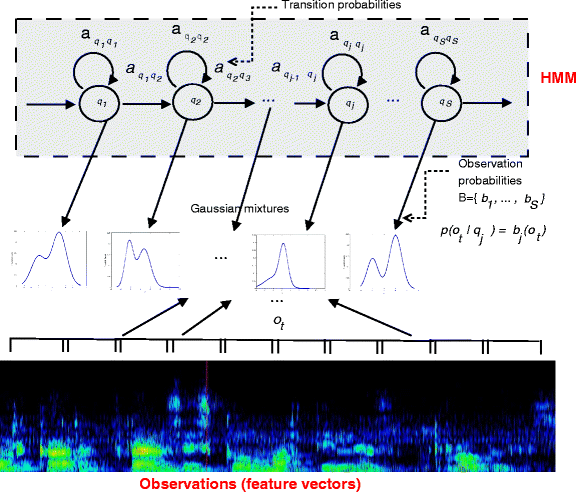
\includegraphics[width=0.75\linewidth]{images/GMM_HMM_diagram.png}
	\caption{Image by \cite{HMM_GMM_image}}
\end{figure}

\noindent Δημιουργούμε ένα HMM ανά ψηφίο, οπότε η έξοδος του i-οστού HMM θα είναι η πιθανότητα το σήμα να αντιστοιχεί στο i-οστό ψηφίο. Οι παρατηρήσεις σε κάθε state του HMM είναι ένα διαφορετικό mixture of gaussians. Αφού εκπαιδευτεί το GMM από μόνο του σε όλα τα δεδομένα, θα εκπαιδευτεί από κοινού το GMM-HMM μοντέλο και το μείγμα κατανομών ανά state θα γίνει fit στην παρατήρηση που συμβαίνει σε αυτό το state. Ιδανικά, θα θέλαμε εξ'αρχής να μην εκπαιδεύουμε το GMM σε όλα τα δεδομένα, αλλά μόνο σε αυτά που αντιστοιχούν στο χρονικό διάστημα που περιγράφεται από το state. Κάτι τέτοιο, όμως, είναι δυστυχώς δύσκολο να γίνει, αφού δεν είναι προκαθορισμένο για κάθε ψηφίο το πότε θα γίνει η μετάβαση από το ένα state στο επόμενο, οπότε θα αρκεστούμε στην διαφοροποίηση μεταξύ των GMMs που κάνει στη συνέχεια η από κοινού εκπαίδευση. Τέλος, σημειώνουμε ότι με το μείγμα γκαουσιανών μοντελοποιούμε την κατανομή των MFCCs ανά ψηφίο και state, αφού περιμένουμε πως η κάθε τέτοια κατανομή δεν θα είναι unimodal στον χώρο των MFCCs λόγω των διαφορών στην εκφώνηση του ίδιου ψηφίου μεταξύ διαφορετικών ομιλητών.\\
\\
\noindent Η συνάρτηση train φαίνεται παρακάτω:

\lstinputlisting[language=Python, firstline=239, lastline=249]{../../lab.py}

\noindent Την \verb*|initialize_and_fit_normal_distributions| καθώς είναι υποπερίπτωση του GMM για n\_mixtures = 1.\\
\\
\noindent Η αρχική εκπαίδευση του GMM γίνεται ως εξής:

\lstinputlisting[language=Python, firstline=165, lastline=175]{../../lab.py}

\noindent Δηλαδή αρχικοποιούμε κάθε γκαουσιανή σε multivariate gaussian με μέσο ειλημμένο από D-διάστατη τυπική κανονική κατανομή, όπου D η διάσταση των δεδομένων, εδώ 13 για τα MFCCs, και με συνδιασπορά τον D-διάστατο ταυτοτικό πίνακα. Επίσης περιορίζουμε κατά την εκπαίδευση τον πίνακα συνδιασποράς να είναι διαγώνιος, ώστε να μειώσουμε τις παραμέτρους και τον χρόνο εκπαίδευσης αλλά και να έχουμε πιο απλές αναπαραστάσεις για τα δεδομένα μας.\\
\\
\noindent Αντίστοιχα, το HMM το εκπαιδεύουμε ως εξής:

\lstinputlisting[language=Python, firstline=220, lastline=236]{../../lab.py}

\noindent Για πίνακα μετάβασης χρησιμοποιήσαμε τον $A = [α_{i, j}]_{1 \le i, j \le n}$, όπου $n = \text{n\_states}$ το πλήθος καταστάσεων στα HMMs, με:
$$α_{i, j} = 
\begin{cases}
	1, & \text{if $j = i = n$}\\
	0.8 & \text{if $j = i \neq n$}\\
	0.2 & \text{if $j = i+1$}\\
	0 & \text{αλλιώς}
\end{cases}
$$

\noindent Οι τιμές 0.8 για την ανακύκλωση και 0.2 για την μετάβαση επιλέχθηκαν επειδή το μοντέλο πιο συχνά θα επιλέγει να μείνει στην ίδια κατάσταση, παρά να μεταβεί στην επόμενη. Επιπλέον, στον κώδικά μας, επειδή η βιβλιοθήκη pomegranate δημιουργούσε nan values από αριθμητική αστάθεια κατά την εκπαίδευση, βρήκαμε ότι αν στον τελευταίο κλάδο (otherwise) θέσουμε $α_{i, j} = ε$ για κάποιο μικρό $ε > 0$ αντί για $0$, σταματούσε το πρόβλημα αφού υπήρχε καλύτερη αριθμητική ευστάθεια.\\
\\
\noindent Τέλος, αρχικοποιήσαμε τις πιθανότητες εκκίνησης ως $1$ στην αρχική κατάσταση και $0$ σε όλες τις άλλες, ενώ τις πιθανότητες τερματισμού ως $1$ στην τελική κατάσταση και $0$ σε όλες τις άλλες.

\lstinputlisting[language=Python, firstline=204, lastline=217]{../../lab.py}